\section{Preliminary analysis}
\label{sec:results}

Using the available data, I conducted an initial descriptive analysis focusing primarily on government advertising spending. To start, I constructed a panel dataset of media outlets that received government funds both before and after the spending reduction. This approach was adopted due to time constraints, but further analysis will be needed to identify which outlets started receiving funds after AMLO’s spending cuts, which outlets ceased to exist, which ones stopped receiving funds, and which ones were newly established. These factors are crucial for constructing a balanced panel dataset. From this I was able to obtain a few descriptive statistics of the data.

The total number of distinct media outlets (newspapers) I was able to identify is 97. Of these, 65 experienced a decrease in advertising spending when comparing before 2019 to after, while the remaining 32 saw an increase. Importantly, the decrease among the 65 outlets was not only more widespread but also significantly larger in magnitude than the total increase observed in the other outlets. This is evident in Table \ref{tab:top_losers}, which lists the top 10 earners during both periods. Overall, there was a noticeable decline in spending at the top end of the distribution. However, most of the top-earning outlets before the decrease remained top earners after the reduction, suggesting that the decline was more generalized rather than selectively targeted.

\begin{table}

\caption{Top 10 Advertisement Earners Before and After (in millions of Mexican pesos)}
\label{tab:top_losers}
\centering
\begin{tabular}[t]{cc | cc}
\hline
\textbf{Outlet} & \textbf{Spending (Before)} & \textbf{Outlet} & \textbf{Spending (After)}\\
\hline
El Universal & 304.3 & La Jornada & 97.4\\
La Jornada & 128.8 & Medios Masivos Mexicanos & 81.2\\
El Financiero & 82.9 & El Universal & 52.6\\
Milenio & 82.5 & Milenio & 43.1\\
Medios Masivos Mexicanos & 75.9 & Reforma & 33.9\\
El Economista & 70.6 & E y P de Medios de los Estados & 32.1\\
La Crónica Diaria & 68.1 & Grupo Cantón & 25.2\\
La Razón de México & 64.1 & El Economista & 20.6\\
Expansión & 62.2 & Azteca Noticias & 18.1\\
El Sol de México & 60.8 & El Financiero & 17.6\\
\hline \\[-1.8ex]  \multicolumn{4}{l} {\parbox[t]{18cm}{\scripsize \textit{Notes:}  Descriptive statistics of the COMSOC advertising spending dataset. The period before refers to the years 2017 and 2018, while the period after refers to 2019 and 2020. All numeric variables are in millions of Mexican pesos. At that moment 1USD $\approx$ 19MXN on average.}} \\
\end{tabular}
\end{table}

On the other hand, some new outlets reached the top 10, such as Grupo Cantón, who is a known aligned media outlet. However, it is unclear if they became aligned after this switch, or were aligned with MORENA even before. Table \ref{tab:earners} presents the top earners from the increases and decreases. Two observations stand out. The first one being that there was a significant percentage increase to some outlets, mostly because they were not receiving relatively any funds before. These outlets that saw the highest percentage increases, such as Proceso, Editorial Golfo Pacífico, and Editora de Medios Mapa, were among those previously receiving relatively low government spending. Furthermore, these media outlets are far from aligned, for instance, AMLO referred to Proceso as engaging in "\textit{conservative journalism, serving corrupt minorities, either directly or indirectly, consciously or unconsciously}" \citep{Attack-Proceso}. 

Moreover, they manage multiple local newspapers, particularly in historically neglected regions, such as southern Mexico (Oaxaca, Chiapas, Campeche, etc.). This suggests a shift in funding from large national outlets, like El Universal, to smaller, local outlets, such as Noticias y Voz de Oaxaca (owned by Golfo Pacífico). Second, many outlets lost over 80\% of their government revenue, a big blow to their finances, especially considering that their largest client is the government. This goes in favor of the hypothesis set up at the beginning, as such a significant redistribution of funds likely influenced the behavior of these outlets. 

\begin{table}

\caption{Top Earners and Losers after the Reform (in millions of Mexican pesos)}
\label{tab:earners}
\centering
\begin{tabular}[t]{cc|cc}
\hline
\textbf{Outlet (Winners)} & \textbf{Total Change} & \textbf{Outlet (Losers)} & \textbf{Total Change}\\
\hline
E y P de Medios de los Estados & 27.8 (645\%) & El Universal & -251.6 (-83\%) \\
Grupo Cantón & 25.0 (10,652\%) & El Financiero & -65.3 (-79\%) \\
El Reforma & 9.9 (41\%) & La Crónica Diaria & -63.6 (-93.5\%) \\
Proceso & 5.3 (207\%) & Expansión & -60.2 (-97\%)\\
Medios Masivos Mexicanos & 5.3 (6.9\%) & La Razón de México & -58.9 (-92\%)\\
Azteca Noticias & 4.4 (32\%) & El Sol de México & -55.5 (-91\%)\\
Editorial Golfo Pacífico & 3.8 (1979\%) & El Economista & -49.9 (-70.7\%)\\
Stereorey México & 2.8 (2172\%) & Milenio & -39.4 (-47.7\%)\\
Piedra Angular & 1.8 (55.3\%) & Información Integral & -35.5 (-87.6\%)\\
Editora de Medios Mapa & 1.7 (1250\%) & TV Notas & -34.7 (-87\%)\\
\hline \\[-1.8ex]  \multicolumn{4}{l} {\parbox[t]{18cm}{\scripsize \textit{Notes:}  Descriptive statistics of the COMSOC advertising spending dataset. The period before refers to the years 2017 and 2018, while the period after refers to 2019 and 2020. Each even column represents the total change in advertising spending from the 2017-2018 period to the 2019-2020, with the percent change it represented. All numeric variables are in millions of Mexican pesos. At that moment 1USD $\approx$ 19MXN on average.}} \\
\end{tabular}
\end{table}

In addition, I compiled and analyzed crime incidence data from the Executive Secretariat of the National Public Security System (\textit{Secretariado Ejecutivo del Sistema Nacional de Seguridad Pública}, SESNSP). This data captures alleged crimes recorded in preliminary investigations or inquiry files, reported by the Offices of the Attorneys General and General Prosecutors at the state level for common jurisdiction crimes and by the Office of the Attorney General of the Republic for federal jurisdiction crimes. The dataset is reported monthly and includes all Mexican municipalities from 2015 to 2024.

For this analysis, I focused on reported homicides between 2015 and 2022. Figure \ref{fig:homicides} presents the monthly trend in reported homicides. Notably, there was a significant rise in homicides during the final years of Peña Nieto’s presidency, peaking around 2017, with levels remaining persistently high through 2020. This suggests that violence had already reached historical highs during this period, which could indicate that media outlets should have increased coverage of violence.

\begin{figure}[h]
   \centering
   \caption{Evolution of monthly reported homicides (2015-2023)}
   \label{fig:homicides}
   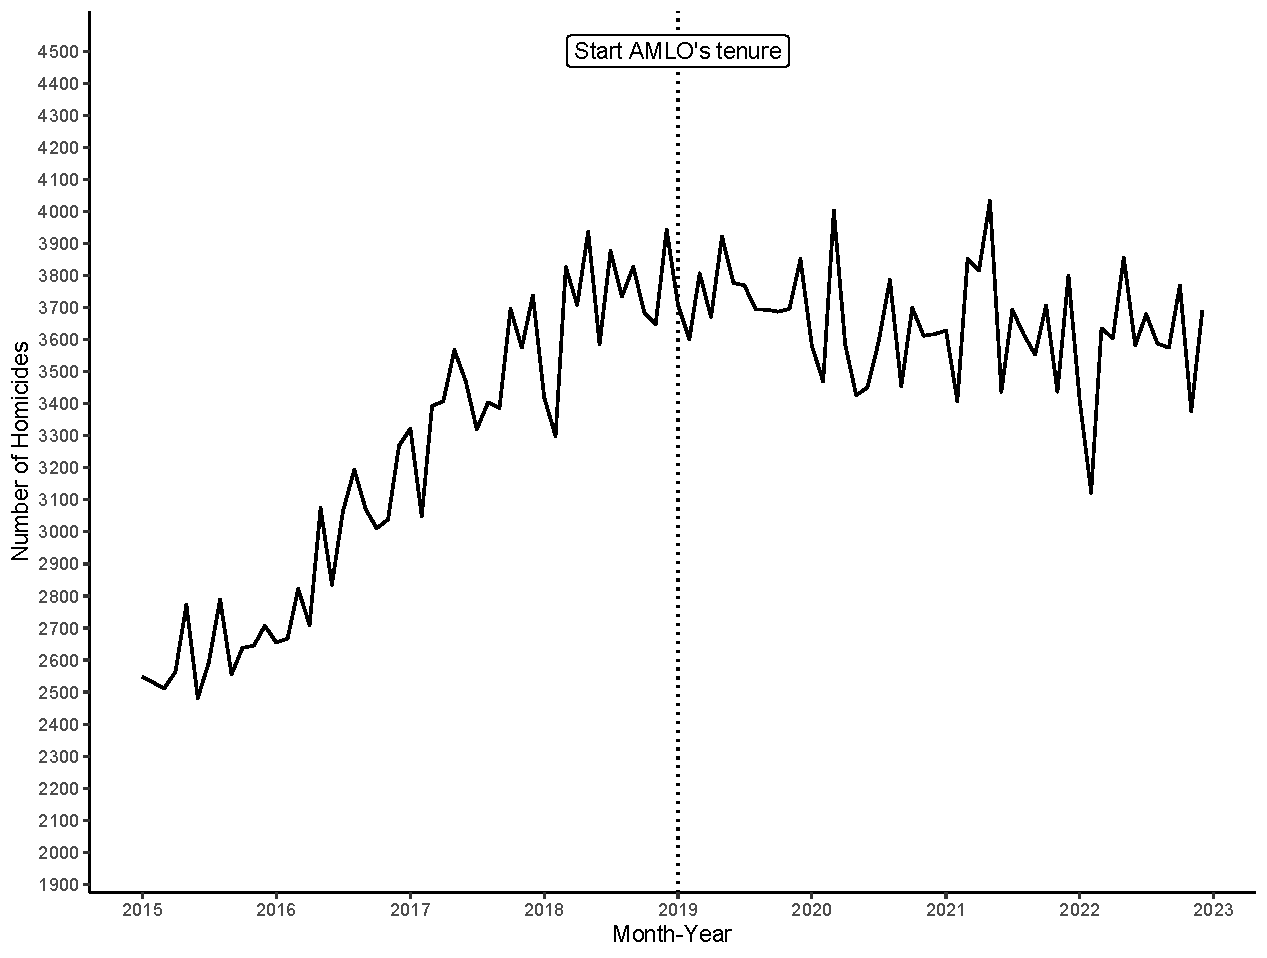
\includegraphics[width=.9\textwidth]{figures/descriptive_stats/homicides.pdf}
   \caption*{ \footnotesize{\textit{Note:} This figure presents the monthly line trend (2015-2023) for the homicide incidence. The black horizontal line represents the start of AMLO's tenure. Data was obtained from SENSNP.}}
\end{figure}

However, while the overall levels of violence in both periods might appear comparable, there could have been a shift in its geographic distribution, with some areas becoming new hotspots while violence decreased in others. Figure \ref{fig:maps} illustrates the geographic distribution of violence before and after the changes in advertising spending, highlighting potential shifts in regional hotspots. As we can see, the distribution of hotspots is fairly similar across time periods, with most of the violence focused on the northern regions closed to the border and the coasts of Guerrero and Jalisco. However, there is a significant increase in violence in the southeastern part of Mexico, particularly focused on Quintana Roo and Campeche, while a decrease in Baja California Sur. Overall, although the time periods are not entirely different evidence would suggest in favor of analyzing the change in coverage leveraging also geographical changes in state violence, that could potentially affect the parallel trends assumption and in consequence the validity of my causal estimates.

\begin{figure}[!htpb]
   \centering
    
   \small
   \caption{Distribution of homicides across the country by municipality}
  \label{fig:maps}
   \caption*{(a) (2017-2018)}
   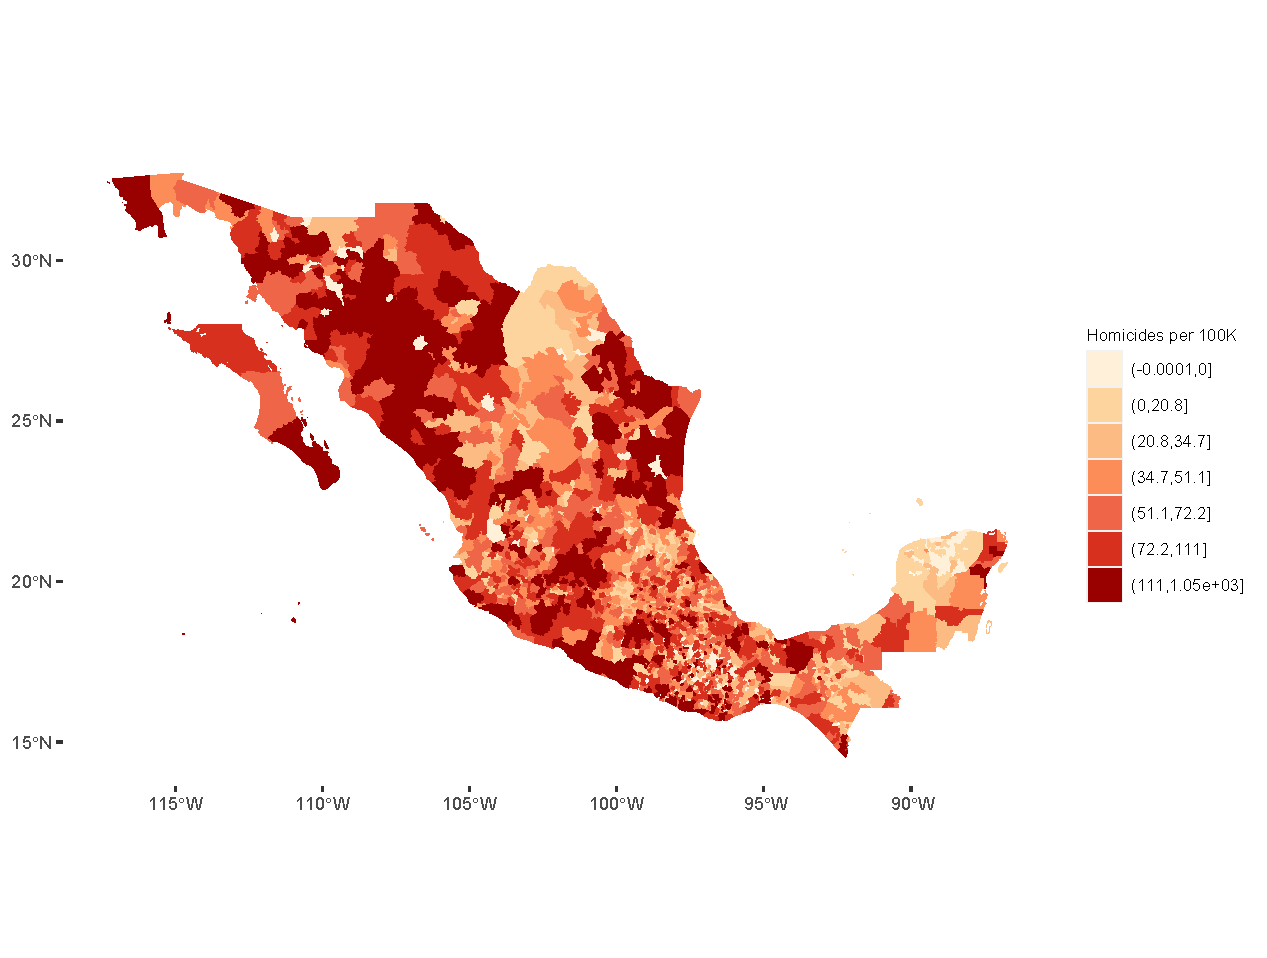
\includegraphics[width=.8\textwidth]{figures/descriptive_stats/map_homicides_before.pdf}
   
   \vspace{1em} % Add spacing between the two figures

    % Second figure
    \caption*{b) (2019-2020).}
    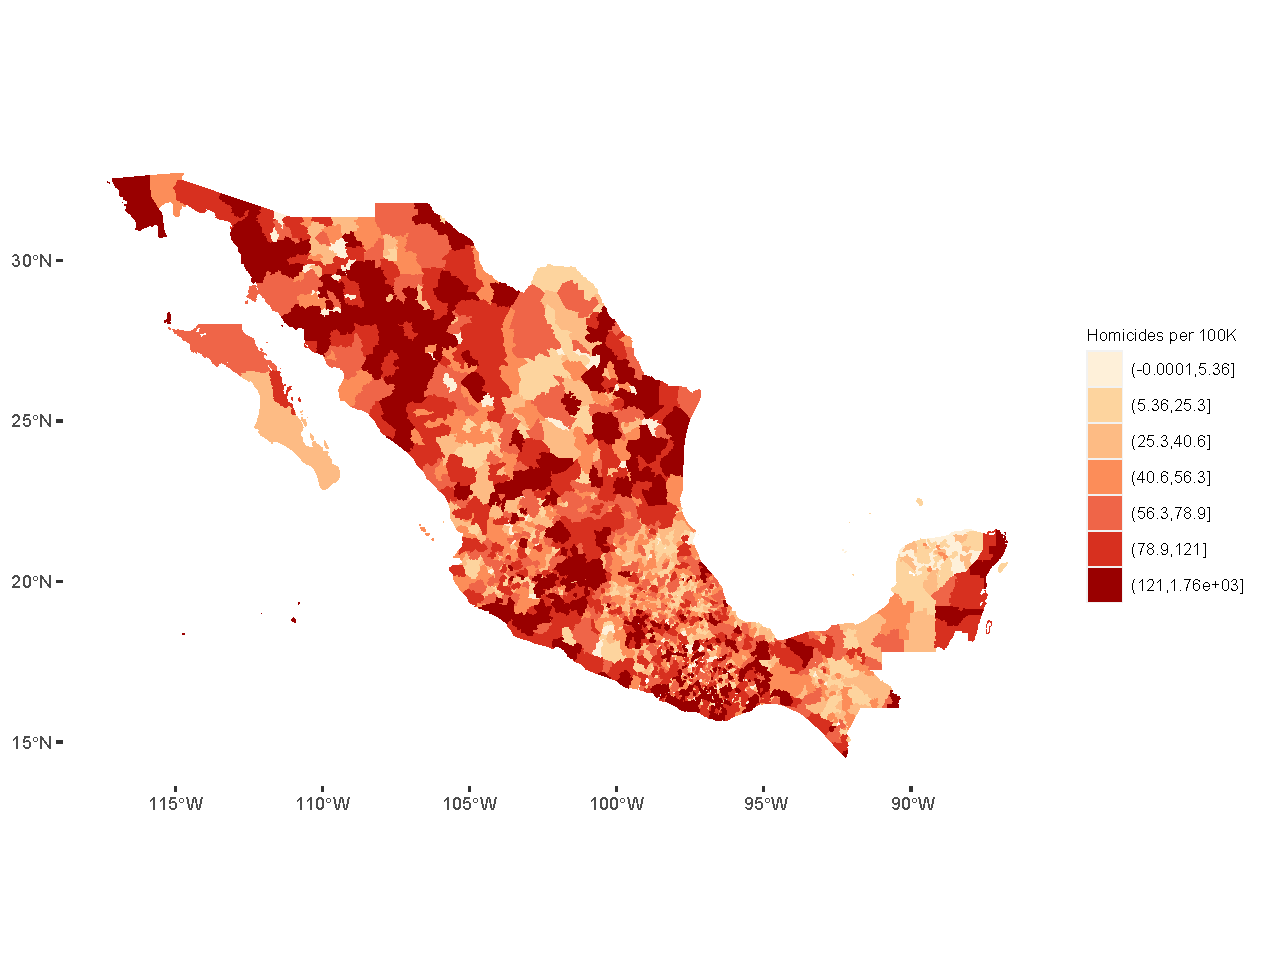
\includegraphics[width=0.8\textwidth]{figures/descriptive_stats/map_homicides_after.pdf} % Replace with your image file
     % Sub-caption for the second figure
\end{figure}
\newpage